\section{Verificação e Seleção do Trocador de calor}

Os critérios selecionados para análise do trocador de calor foram definidos visando garantir que o projeto atendesse às exigências de desempenho e eficiência térmica. Com base nos resultados obtidos anteriormente, os parâmetros estabelecidos são:

\begin{enumerate}
	\item \textbf{Área de Transferência de Calor}: A área de troca térmica deve ser maior que 2,16 m². Este critério é essencial para assegurar que o trocador de calor tenha capacidade suficiente para realizar a transferência de calor necessária entre os fluidos, atendendo à demanda do processo.
	
	\item \textbf{Vazão de Óleo}: A vazão mínima do óleo deve ser superior a 35,7 L/min. Este valor foi definido para garantir que o fluido tenha uma taxa de fluxo adequada, maximizando a eficiência de troca térmica e prevenindo possíveis pontos de estagnação no sistema.
	
	\item \textbf{Potência Térmica Mínima}: A potência mínima deve ser inferior a 37,6 kW, o valor de \( Q_{real} \) obtido nos cálculos. Este limite inferior garante que o trocador possa operar adequadamente sem ultrapassar a carga mínima necessária para o sistema.
	
	\item \textbf{Potência Térmica Máxima}: A potência máxima deve ser superior a 63 kW, o valor de \( Q_{max} \) calculado. Esse critério assegura que o trocador de calor possui capacidade suficiente para suportar picos de demanda térmica, evitando perda de eficiência em condições de operação máxima.
\end{enumerate}

Esses critérios foram definidos para assegurar a robustez e a eficiência do trocador de calor, considerando tanto a operação regular quanto as possíveis variações no processo. Eles também servem como parâmetros para futuras revisões de desempenho e manutenção do sistema.

Porém, ao comparar os dados com a tabela de modelos disponíveis, verificou-se o seguinte padrão:

\begin{figure}[h]
	\centering
	\caption{Valores da tabela de trocadores de calor, classificados em verde como "ok" para atendimento dos requisitos e em vermelho para "desacordo" com o projeto}
	\label{fig:screenshot001}
	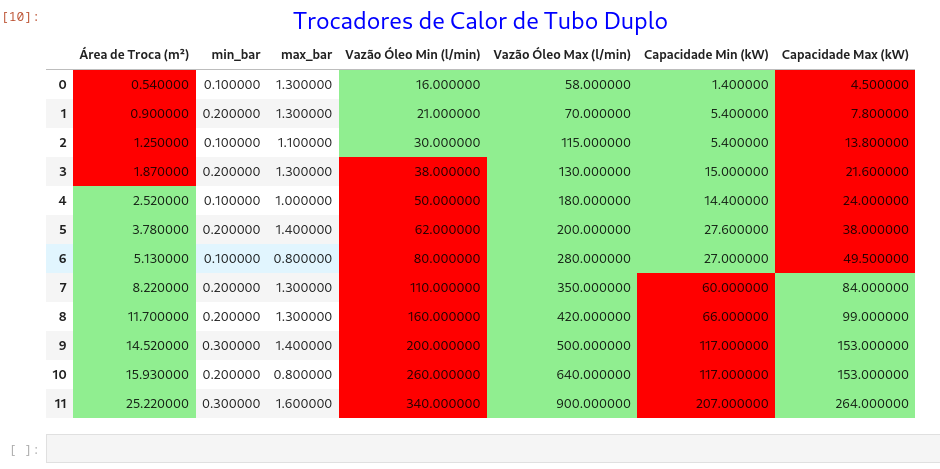
\includegraphics[width=1\linewidth]{imagens/screenshot001}
	
	\text{Fonte: Elaborado pelos autores (2024)}
\end{figure}

Logo, nenhuma das opções demonstrou-se viável para o projeto. Qualquer tentativa de utilizar algum dos trocadores de calor disponíveis, irá requerer alterações em seus projetos ou em adaptações (não recomendadas) em seus padrões de operação que podem vir a diminuir a vida útil e/ou tornar a manutenção mais onerosa do que o necessário.
